\documentclass[UTF8]{ctexart}
\usepackage{graphicx}
\usepackage{float}
\usepackage{url}
\usepackage{geometry}
\usepackage{fancyhdr}
\usepackage{lastpage}
\usepackage{amsmath}
\usepackage{booktabs}
\usepackage{multicol}
\usepackage{multirow}
\usepackage{color}
\usepackage{subfigure}
\usepackage{listings}
\geometry{left=2.54cm,right=2.54cm,top=3.18cm,bottom=3.18cm}%页边距
\pagestyle{fancy}
\lhead{
\includegraphics[scale=1]{sjtu-logo-red.pdf}}  
\rhead{mini-PACS系统的搭建} 
\cfoot{第 \thepage\ 页\ 共 \pageref{LastPage} 页}   

\lstset{
    basicstyle          =   \sffamily,          % 基本代码风格
    keywordstyle        =   \bfseries\color{blue},          % 关键字风格
    commentstyle        =   \rmfamily\itshape,  % 注释的风格,斜体
    stringstyle         =   \ttfamily,  % 字符串风格
    flexiblecolumns,                % 别问为什么,加上这个
    numbers             =   left,   % 行号的位置在左边
    showspaces          =   false,  % 是否显示空格,显示了有点乱,所以不现实了
    numberstyle         =   \zihao{-5}\ttfamily,    % 行号的样式,小五号,tt等宽字体
    showstringspaces    =   false,
    captionpos          =   t,      % 这段代码的名字所呈现的位置,t指的是top上面
    frame               =   lrtb,   % 显示边框
}

\begin{document}
\bibliographystyle{unsrt}
\begin{titlepage}
    \begin{center}
        
\includegraphics[width=0.8\textwidth]{sjtu-name-blue.pdf}\\[1cm]
        \textsc{\Huge \bfseries 课程报告}\\[1.5cm]
        
\includegraphics[width=0.3\textwidth]{sjtu-badge-blue.pdf}\\[0.5cm]

        \Huge \bfseries{mini-PACS系统的搭建}\\[1cm]
        \Large \bfseries{518021910971 裴奕博}
    \end{center}
\end{titlepage}
\tableofcontents
\newpage

\begin{abstract}
    中文摘要
    \textbf{Keywords:} 关键字
\end{abstract}
%正文
\section{开源软件的选择}
\subsection{SCP的选择}
在上次的开源软件调研报告中,我了解到了几个目前流行的开源mini-PACS框架,其中就有Orthanc。Orthanc是一个基于C++开发的轻量级mini-PACS框架,采用GPL协议开源。它具有以下几个特点\cite{enwiki:1041672725}:
\begin{enumerate}
    \item 提供了内置的http服务,可以通过Web应用来可视化的上传、查看、检索和传输Dicom文件。
    \item 跨平台。可以在Windows下运行,也可以通过Docker在Linux下运行,可以部署在常见的网站服务器上如Nginx、Apache等。
    \item 可以通过多种方式实现Dicom的传输。不仅提供了Dicom Server端口,也可以使用Web应用可视化上传,更是提供了REST API直接上传Dicom文件。
\end{enumerate}
\begin{figure}[H]
    \centering
    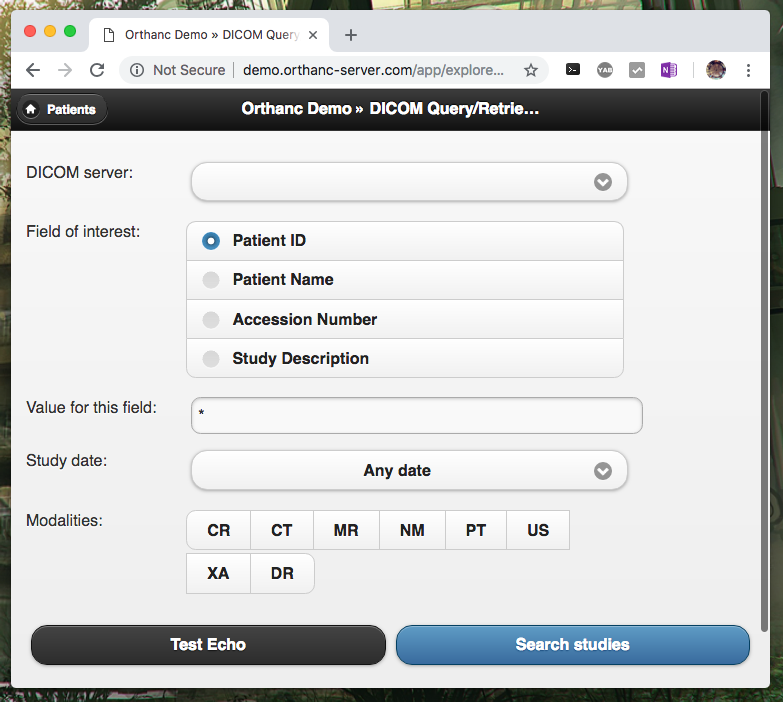
\includegraphics[width=0.4\textwidth]{orthanc.png}
    \caption{Orthanc界面}
    \label{fig:Orthanc}
\end{figure}

Orthanc目前仍然在持续更新中,更加现代化,界面也漂亮舒适。因此在本次实验中选择了Orthanc作为Dicom服务器。

\subsection{SCU的选择}
由于Orthanc提供了多种传输方式,因此此次实验既尝试使用了开源的DCMTK作为SCU,也尝试了直接使用Web应用上传。

DCMTK是由德国offis公司提供的开源项目,使用C++实现了Dicom协议的相关细节,并封装成了各个应用,为我们提供了实现DICOM协议的一个平台,使得我们可以在它的基础上轻松的完成自己的主要工作,而不必把太多的精力放在实现DICOM协议的细节问题上\cite{DCMTKbaidu}。实际上,Orthanc的后端也集成了DCMTK工具包用于Dicom文件的相关操作。

\section{mini-PACS系统的搭建}
\subsection{Server的配置}
根据Orthanc的官方文档\cite{OrthancBook},Orthanc在安装完毕时即提供了默认配置,包括默认的sqlite数据库、默认的Dicom服务、默认的http服务及其端口,因此只需要修改自己需要的部分,其他部分均会由Orthanc读取默认配置文件。本次实验采用的配置文件server\_config.json内容如下:

\begin{lstlisting}[language=C]
    {
        "Name": "My archive",
        "HttpPort": 4200,
        "DicomAet": "ARCHIVE",
        "DicomPort": 104
    }
\end{lstlisting}

由于使用了自定义的配置文件,因此启动Orthanc时需要指定配置文件路径。因此使用了bat脚本来方便Server的启动。脚本runOrthanc.bat内容如下:
\begin{lstlisting}[language=C]
    "D:\Program Files\Orthanc Server\Orthanc" ./server_config.json --trace
\end{lstlisting}
参数--trace或--verbose可以提供调试时的相关信息,由于需要观察日志,因此将--trace选项打开。

\subsection{通过Web应用上传Dicom文件}
通过运行上述脚本运行Orthanc,此时http Server端口为4200,Dicom Server端口为104。进入浏览器,输入\url{localhost:4200}进入Orthanc界面,点击顶部的Upload菜单即可进入上传界面。

\begin{figure}[H]
    \centering
    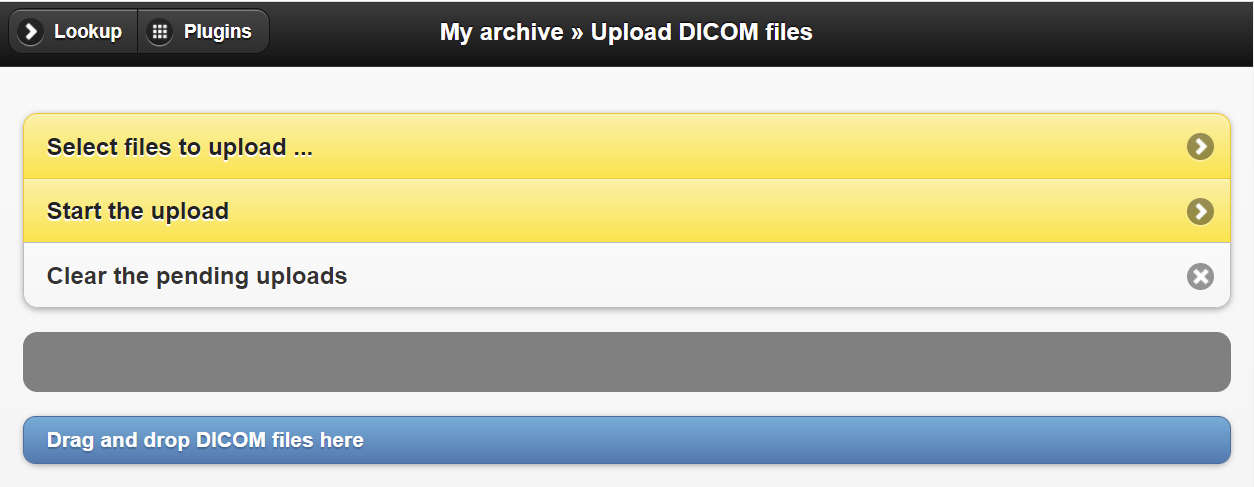
\includegraphics[width=0.6\textwidth]{web upload.png}
    \caption{Orthanc上传界面}
    \label{fig:Orthanc Upload}
\end{figure}

在此界面即可通过拖动和选择文件的方式在图形界面中上传文件。

\subsection{通过DCMTK上传Dicom文件}
上述的方式虽然方便,但需要逐个选择上传的文件。如碰到数据量较大的情况就很不方便。此时可以选择通过DCMTK借助命令行脚本的方式上传。

在DCMTK中,C-STORE的命令被封装在storescu.exe中,通过DCMTK官网的文档,我们可以得知其使用方法\cite{DCMTK}:
\begin{lstlisting}[language=C]
    storescu.exe -d -aec ARCHIVE localhost 104 $file
\end{lstlisting}
命令行参数-d输出调试信息,-aec指定应用实体名字,并指定端口号和上传文件。通过PowerShell脚本(storeDCM.ps1)即可批量上传一个文件夹下的所有DCM文件。足够实现一个序列或者检查的批量上传。
\begin{lstlisting}
    $files= Get-ChildItem -Path .\*.dcm 
    foreach($file in $files)
    {
        storescu.exe -d -aec ARCHIVE localhost 104 $file
    }
\end{lstlisting}

\subsection{检索和查看Dicom文件}
这一部分功能均由Orthanc内置。通过Lookup选项菜单即可查看所有Dicom文件信息。通过病人-检查-序列-实例的层级结构呈现,如下图\ref{fig:Orthanc Lookup}所示。
\begin{figure}[H]
    \centering
    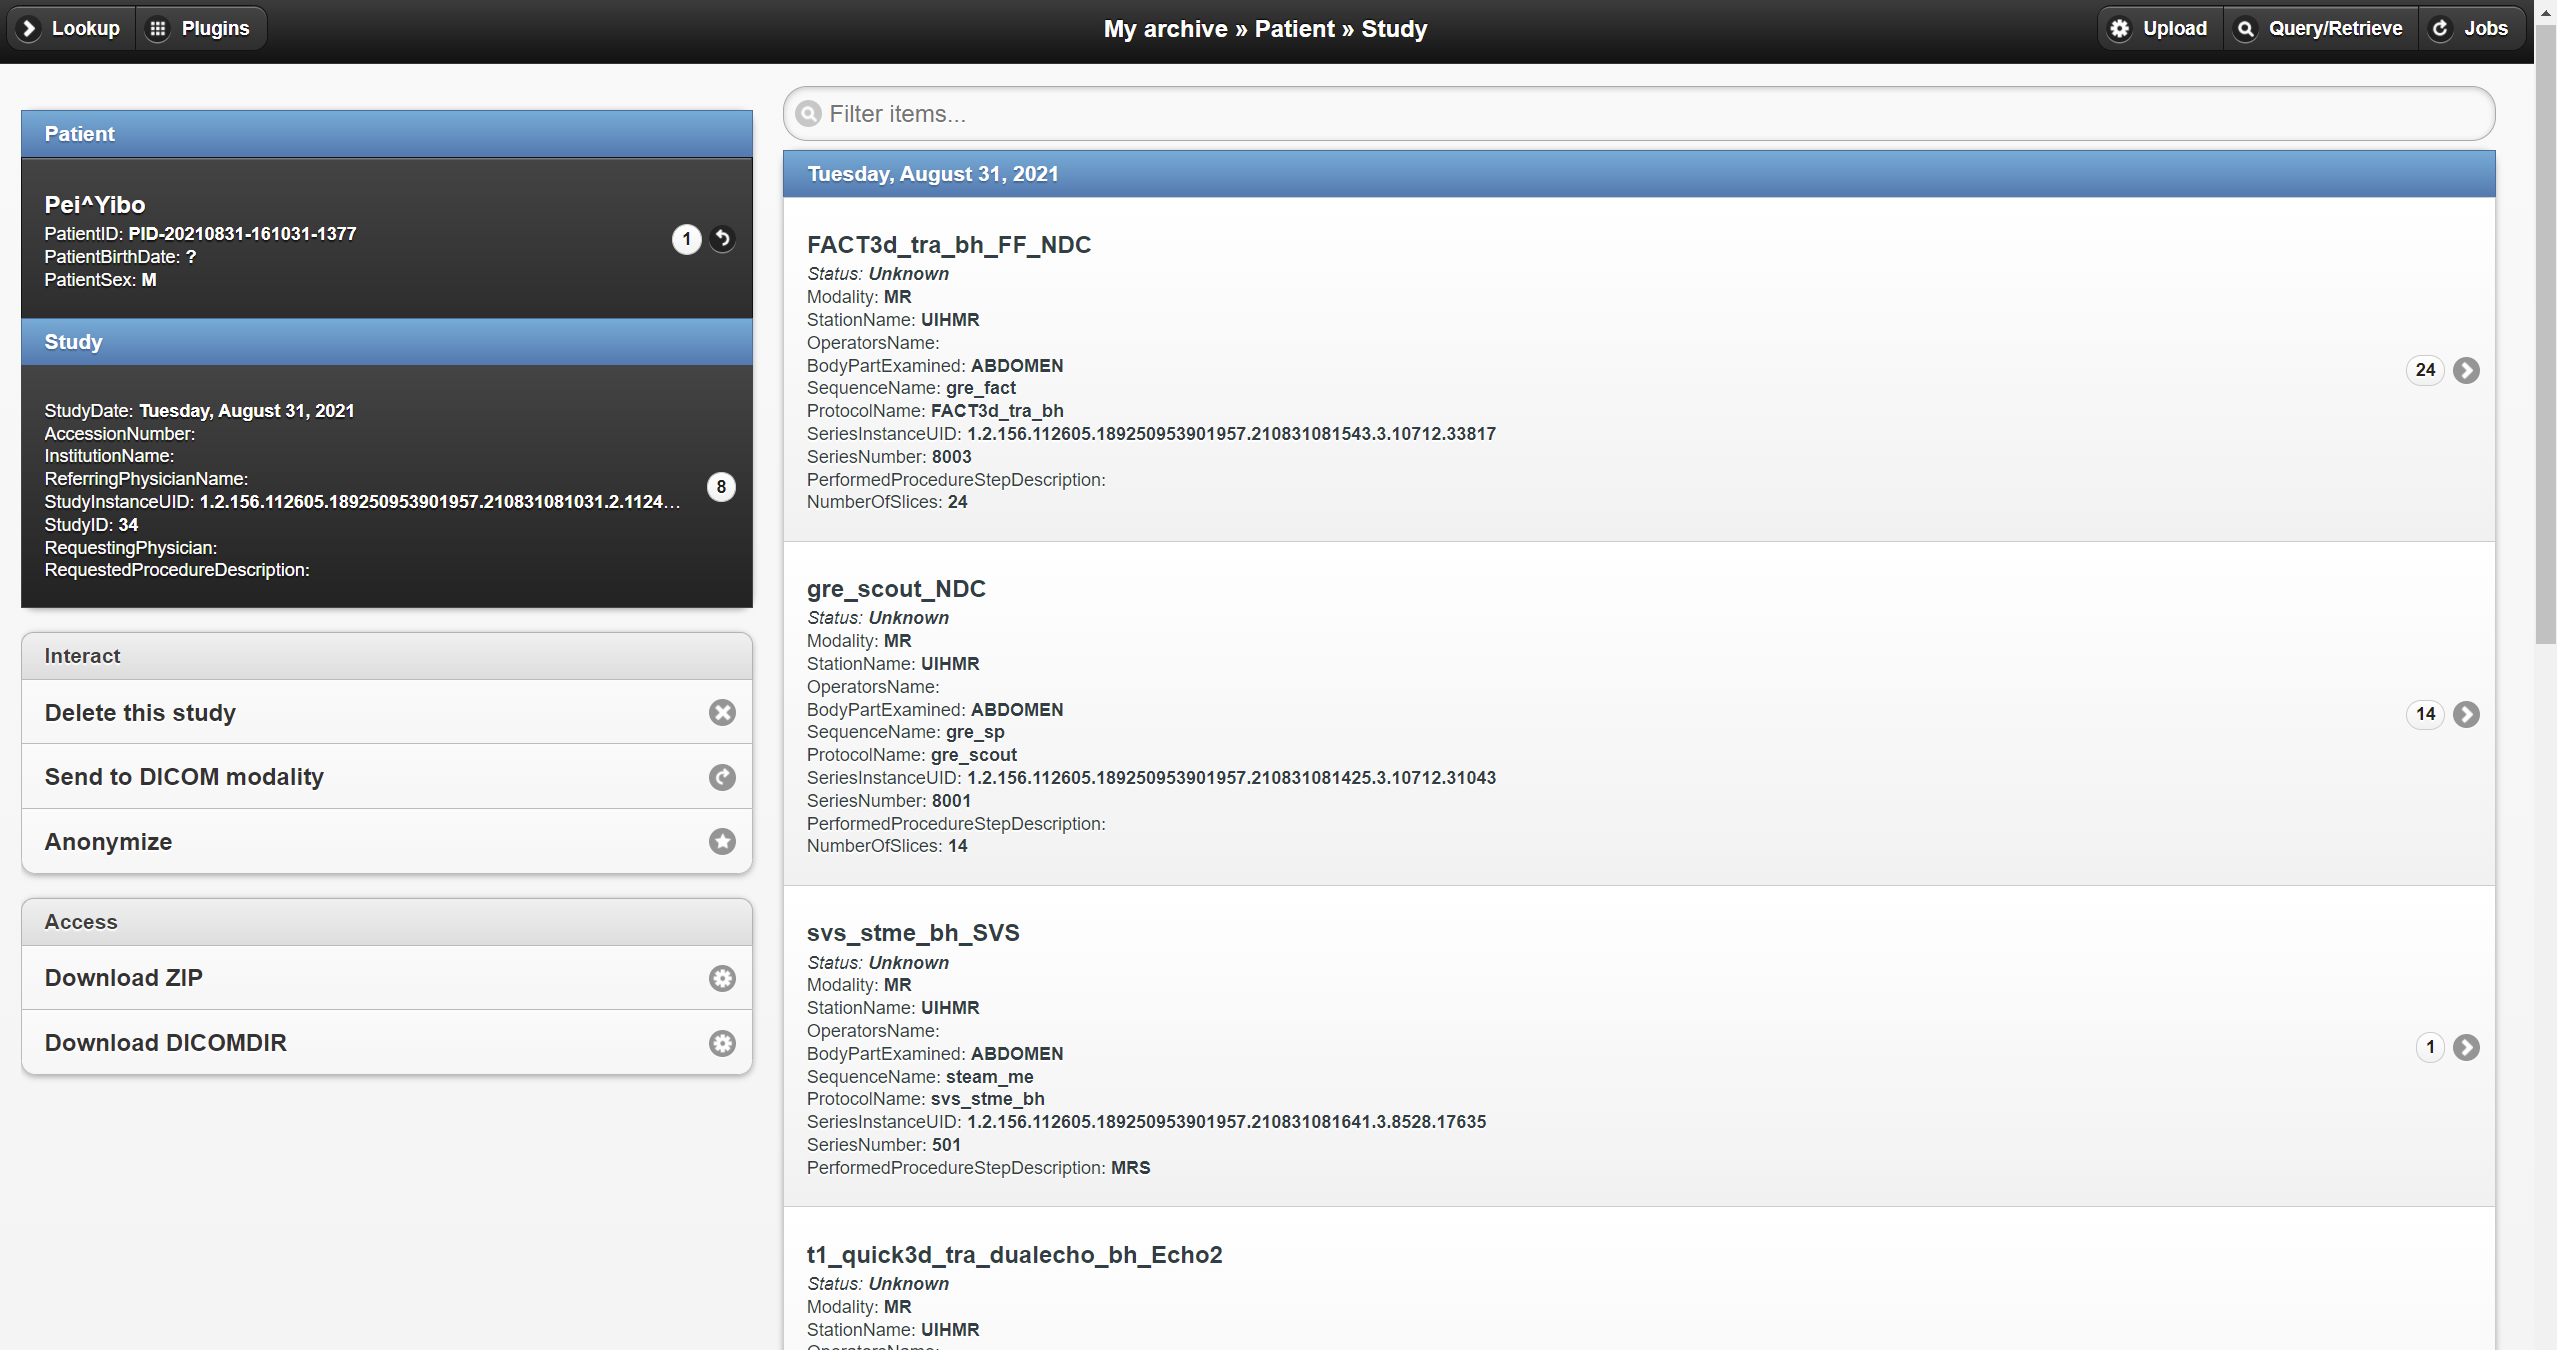
\includegraphics[width=0.8\textwidth]{lookup.png}
    \caption{Orthanc查看界面}
    \label{fig:Orthanc Lookup}
\end{figure}

\section{log日志内容解析}
\subsection{log日志获取}
在VSCode中,打开工作目录,启动Orthanc,使用命令行上传单个Dcm文件,分成两个窗口同时查看SCU和SCP的日志信息\cite{DICOM}:
\begin{figure}[H]
    \centering
    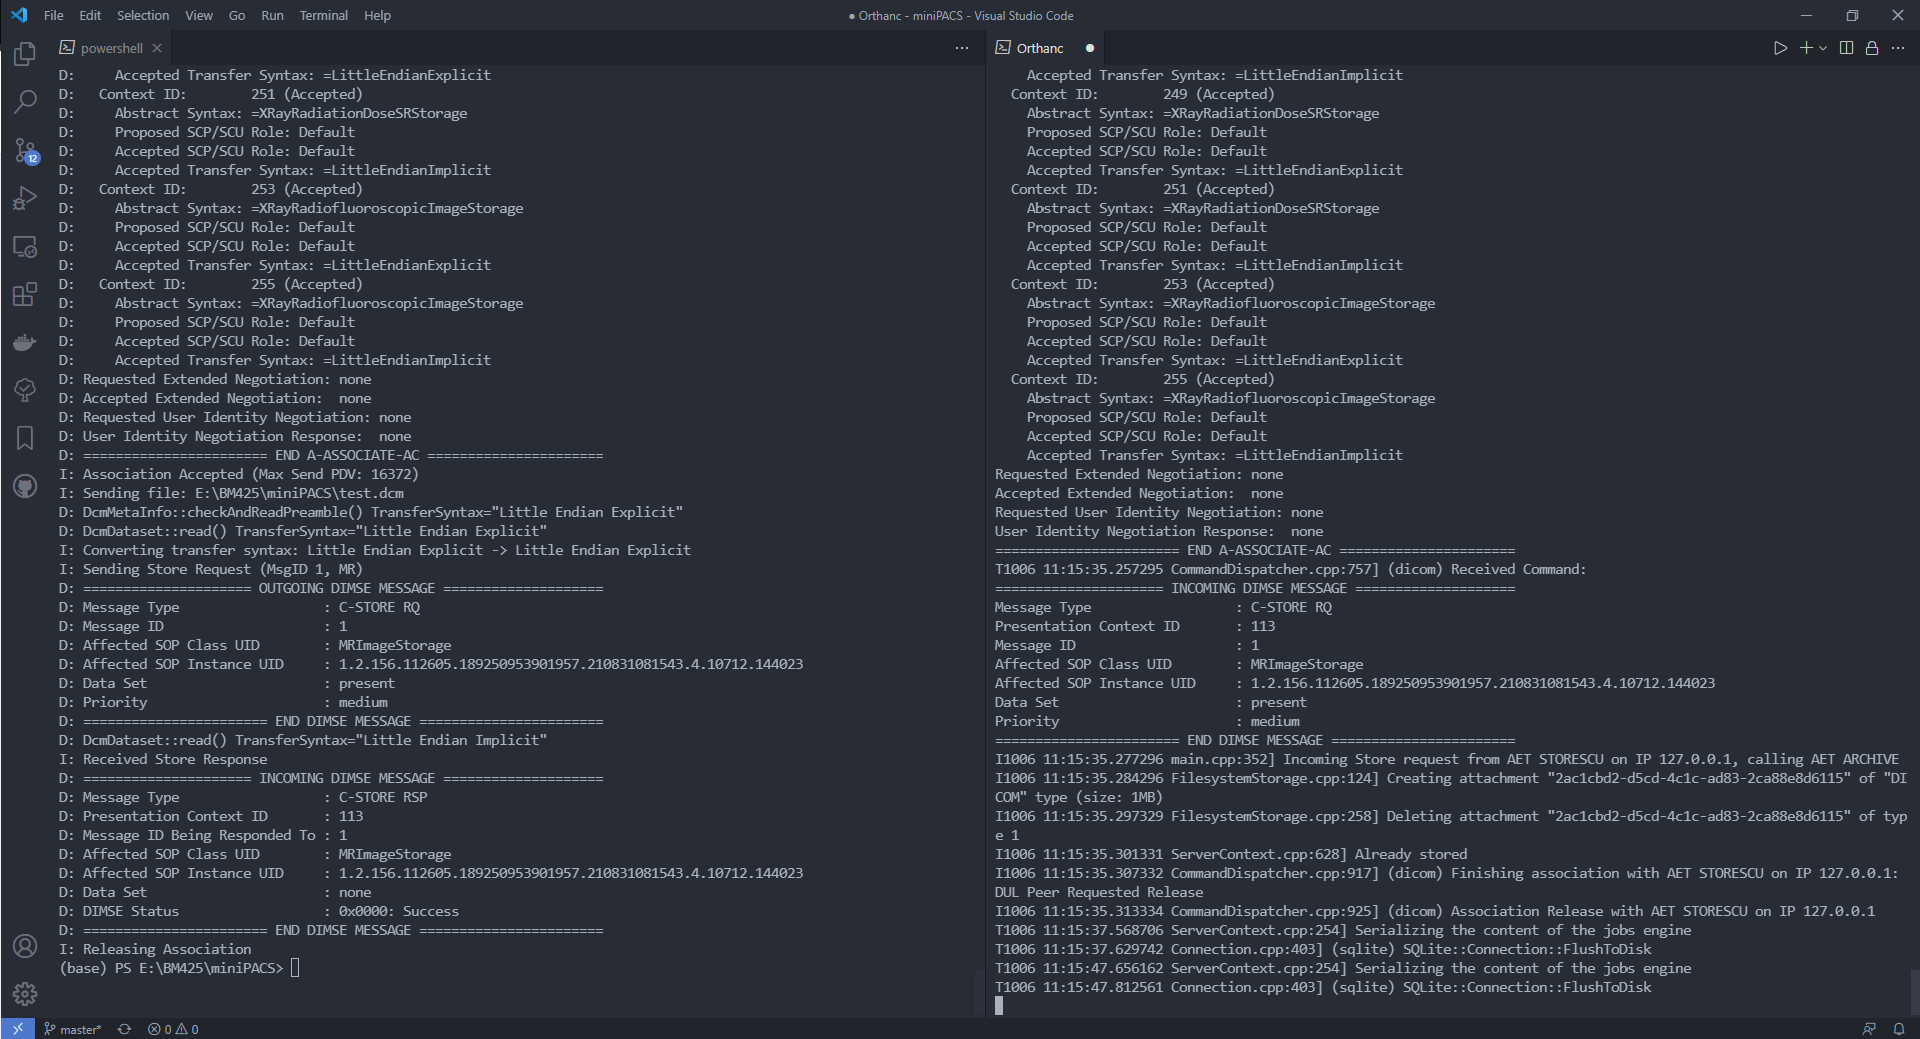
\includegraphics[width=0.6\textwidth]{running.png}
    \caption{log日志获取}
    \label{fig:get log}
\end{figure}
最终得到的日志结果见client\_log.log、server\_log.log和client\_fail\_log.log文本文件。
\subsection{log日志解析}

\begin{table}[H] 
    \centering  
    \caption{\label{tab:test}缩写和名称对照表}   
    \begin{tabular}{ccc}    
        \toprule    
        缩写 & 全称(英文) & 全称(中文) \\    
        \midrule   
        PDU & Protocol Data Units & 协议数据单元 \\   
        DIMSE & DICOM Message Service Element & DICOM消息服务 \\   
        SOP & Service Object Pair & 服务对象对 \\
        \bottomrule   
    \end{tabular}  
\end{table}

无论从SCU还是SCP来看,日志可以分为以下几个部分:
\begin{enumerate}
    \item Associate RQ/AC PDU的交换
    \item DIMSE的发送和接收
    \item 数据在SCP上的存储
\end{enumerate}

\subsubsection{Associate RQ/AC PDU的交换}

这一部分可以分为如下几个步骤:
\begin{enumerate}
    \item SCU生成并发送Associate RQ PDU。
    \item SCP收到Associate RQ PDU后根据状态返回Associate AC PDU(接受连接)或Associate RJ PDU(拒绝连接)。
\end{enumerate}
Associate AC PDU中包含如下信息:
\begin{figure}[H]
    \centering
    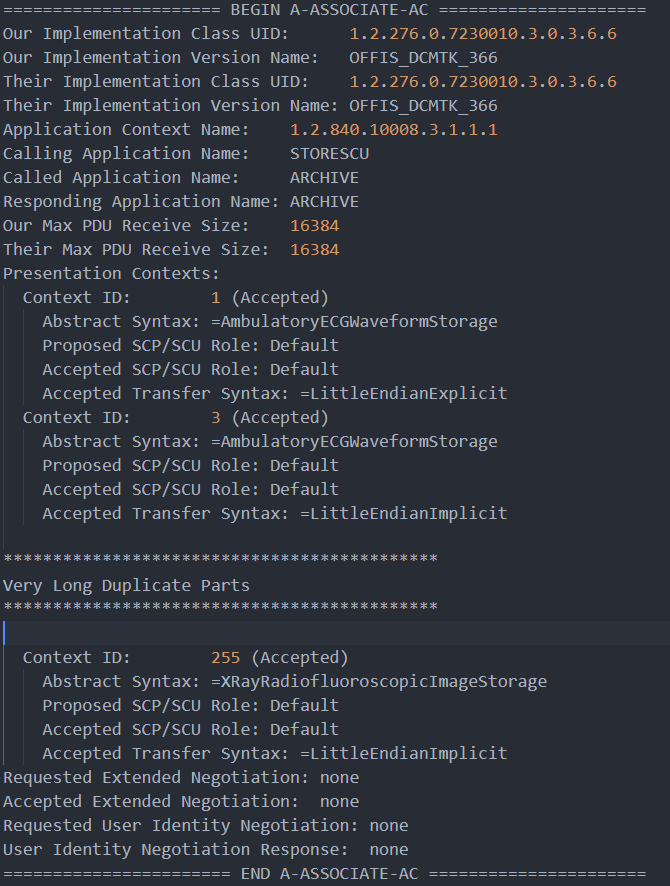
\includegraphics[width=0.6\textwidth]{PDU.png}
    \caption{Associate AC PDU}
    \label{fig: log PDU}
\end{figure}
其中包括协议的class ID,协议实现的版本号,PDU的大小,应用上下文Context等信息。Context共有256段,每段都会返回连接状态(Accepted/Proposed)、Abstract Syntax、SCP/SCU Role等信息。这一部分的信息不包括上传文件的信息,仅供建立连接使用。

\subsubsection{DIMSE的发送和接收}

这一部分可以分为如下几个步骤:
\begin{enumerate}
    \item SCU以OUTGOING DIMSE MESSAGE形式发送一个C-STORE RQ。
    \item SCP收到INGOING DIMSE MESSAGE后根据状态同样以OUTGOING DIMSE MESSAGE形式发送C-STORE RSP给SCU。
    \item SCU收到响应后确认状态,整个STORE流程结束。
\end{enumerate}
这一过程中客户端和服务端的log显示如下:
\begin{figure}[H]
    \centering
    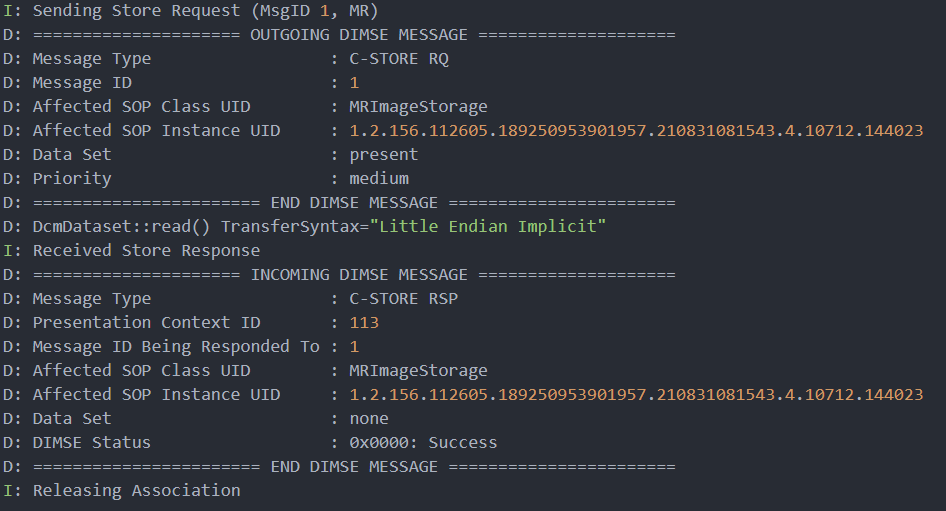
\includegraphics[width=0.6\textwidth]{DIMSE client.png}
    \caption{DIMSE Client Log}
    \label{fig: log Client}
\end{figure}

\begin{figure}[H]
    \centering
    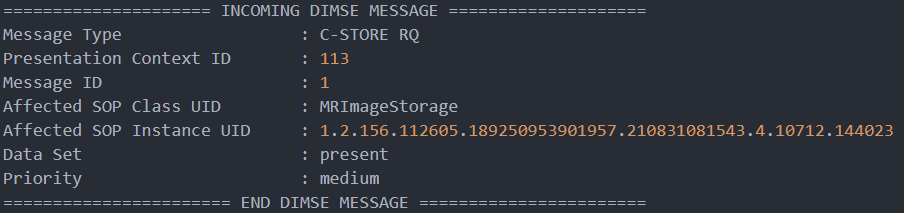
\includegraphics[width=0.6\textwidth]{DIMSE server.png}
    \caption{DIMSE Server Log}
    \label{fig: log server}
\end{figure}
可以清楚的看到SCU和SCP通信时信息的发送和接收。

C-STORE RQ的内容包括以下几个字段:消息类型、消息ID、SOP的类和实例UID、数据集合消息优先级。
C-STORE RSP的内容包括以下几个字段:消息类型、上下文ID、响应对象的ID、SOP的类和实例UID、数据集和DIMSE状态等信息。

最后DIMSE状态若显示为success,则整个DICOM网络通信流程成功进行。

\subsubsection{数据在SCP上的存储}
\begin{figure}[H]
    \centering
    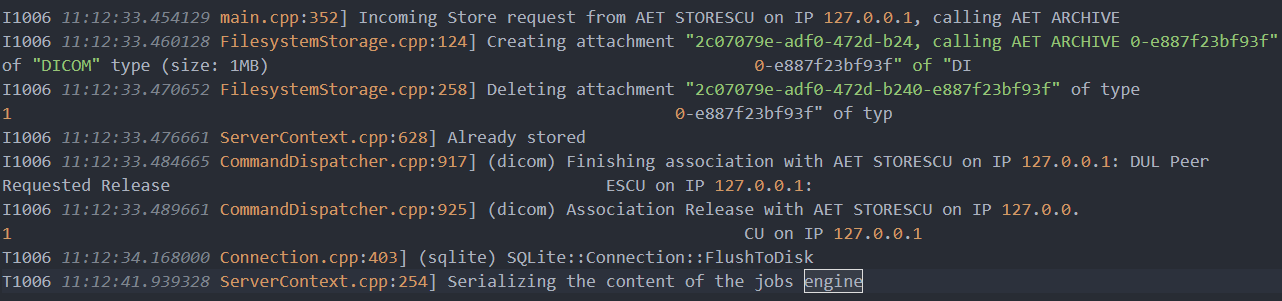
\includegraphics[width=0.6\textwidth]{log store.png}
    \caption{DB Store Log}
    \label{fig: log db}
\end{figure}
在通信流程结束后,Orthanc将上传的Dcm存储到数据库中(此处使用的是默认的sqlite),可在本地的OrthancStorage目录下找到存储的数据。

\section{实验感想}

本次实验尝试使用了现有的开源软件搭建了mini-PACS服务器,并尝试了Dicom文件的上传并查看了日志。在实验过程中,遇到过如下几个问题:
\begin{enumerate}
    \item 端口冲突。在调试时,有时会发现Orthanc由于端口冲突无法启动的情况。\\解决方法:在命令行kill掉占用端口的进程或者修改配置文件换用其他端口号。
    \item 在尝试本地WSL中启动Linux Docker下的Orthanc,模拟实际的远程存储情况时遇到HTTPS encryption is disabled错误。\\ 解决方法:根据官网的提示重新认证证书或使用Nginx,但还未实际实现。
\end{enumerate}

本实验所用的脚本和log文件均已附在压缩包中,附上Orthanc下载地址:\url{https://www.orthanc-server.com/download.php}。

\bibliography{references}
\end{document}
